\section{Mathematical Formulation} 
\label{Problem_definition_formulation}
\subsection{Problem Definition}
A fleet of aircraft is represented by the set $I$, with each aircraft uniquely identified by a tail number $i \in I$. As many different aircraft types (such as Boeing vs Airbus, or wide-body vs narrow-body) are involved in the fleet, the set of all subfleet types, such as 737-800 and A320-Neo, is denoted as $S$. Among all aircraft in fleet $I$, those of subfleet type $s$ are collectively denoted as set $I_s$. Each subfleet type is associated with a set of maintenance checks, or called checks, such as A and C. There are, in total, ten types of C checks (also called phase checks), which are divided into two groups by maintenance interval, namely C01-C06 and C07-C10. The first group is referred to as One-C phase checks, which are conducted more frequently than the phase checks in the second group, namely Two-C phase checks. 
The set of all check types is denoted as $K$. We next define an aircraft-check tuple $w=\left(i,k\right)$ or simply tuple $w$, where $i \in I$ and $k \in K_i$. It is noted that $K_i \subseteq K$ as aircraft $i$ is not required to complete all checks in $K$; only those checks in a subset $K_i$ apply to aircraft $i$.

The maintenance interval for tuple $w=\left(i,k\right)$ is denoted as $m_w$, essentially the maximum possible time (measured in days) between two consecutive checks of type $k$ for aircraft $i$. 
Right after a check is completed, the Days-To-Go or DTG becomes $m_w$,  and it drops by one every day. The initial DTG is denoted as $\delta_w^0$. The next check must be scheduled before the DTG drops to zero (as illustrated in Figure~\ref{fig:maint_cycle}). Otherwise, maintenance is overdue, which is strictly prohibited by FAA regulations. 
Figure~\ref{fig:maint_cycle}  shows and contrasts two possible scenarios: premature vs ideal. In the premature scenario, a check is completed before the DTG drops to the minimum (typically zero or one), and some usable days are then lost or wasted, leading to a yield of less than 100\%. In the ideal scenario, a check is completed on the check due date, and a yield of 100\% is obtained (i.e., zero waste).

% Figure~\ref{fig:maint_cycle} 
% illustrates that when a check is completed before the DTG drops to zero, some usable days are lost or wasted, leading to a yield of less than 100\%. When a check is completed on the check due date, a yield of 100\% is obtained (i.e., zero waste).


\begin{figure}[ht]
    \centering
    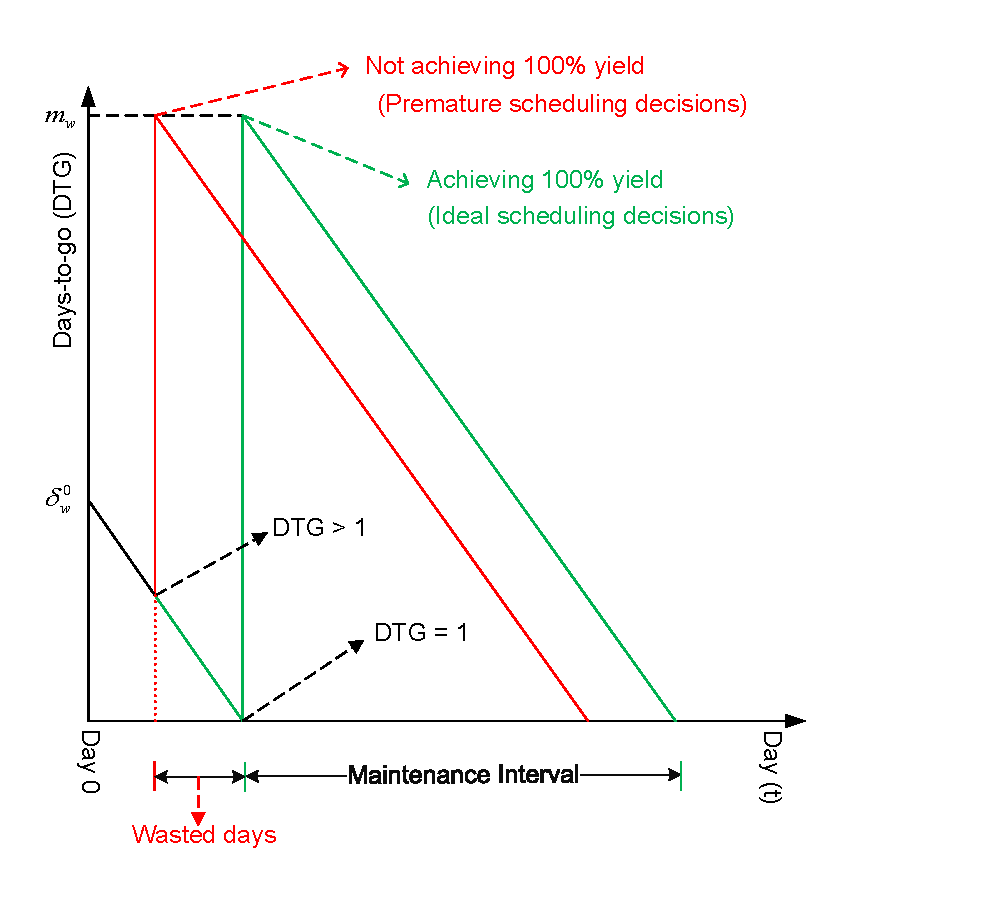
\includegraphics[width=0.65\linewidth]{Daystogo_v2.pdf}    
    \caption{Evolution of days-to-go for a tuple $w$}
    \label{fig:maint_cycle}
\end{figure}


To conduct various checks for all aircraft in the fleet, the airline owns and operates a set of maintenance stations, denoted as $J$. As a station $j \in J$ cannot service all aircraft types, we use $J_w$ to represent a subset of stations that are capable of servicing tuple $w$. Each station $j$ has a few capacity parameters. Specifically, the maximum man-hours available at station $j$ is given as $H_j$; the maximum number of A-checks station $j$ can complete daily is $A_j$; the number of phase checks at station $j$ is limited at $U_j$; the maximum number of phase checks that can be performed on a given aircraft at station $j$ is $R_j$; and the total number of aircraft to be maintained at a station is limited at $Q_j$ each day. When the above capacity parameters vary over time, a superscript $t$ is added. For instance, $H_j$ can be changed to $H_j^t$. Additionally, the number of aircraft of subfleet type $s$ that can access station $j$ on day $t$ for maintenance is limited as $P_{sj}^t$. Note that $\sum_s\sum_jP_{sj}^t$ could be much smaller than the fleet size $|I|$, because not all aircraft could access airports with maintenance capabilities every day. 

As a certain type of aircraft can be maintained at multiple stations, an aircraft has a preference for maintenance stations given its subfleet type due to factors related to routing convenience or historical performance record.  We thus define $\beta_{wj}$ to represent the preference of tuple $w$ for station $j$. For each tuple $w$, a more preferred station $j$ is associated with a lower $\beta_{wj}$, which can also be interpreted as a relative cost. Introducing $\beta_{wj}$ is expected to break the solution symmetry among stations. 

 
Given the fleet of aircraft $I$, its associated maintenance checks $K$, and a set of heterogeneous maintenance stations $J$, the airline seeks to determine on which day $t$ and at which station $j$, which type of check $k$ is scheduled for aircraft $i$. The objective is to minimize the discounted maintenance cost over the planning horizon. 
 

\subsection{Mixed Integer Programming Formulation}
\label{subsec:MIP_formulation}

\begingroup
\setstretch{1} % Set the line spacing to single within this group
\begin{longtable}{l p{16cm}}
\caption{Notation}
\label{tab:notation_tab} \\
\hline
\multicolumn{2}{l}{\textit{Sets and Indices}} \\ \hline
\endfirsthead
\multicolumn{2}{c}{{\tablename\ \thetable{} -- continued from previous page}} \\
\hline
\endhead
\endfoot
\hline
\endlastfoot
$I$ & Set of aircraft, indexed by $i$ \\
$J$ & Set of all maintenance stations, indexed by $j$ \\
$J_i$ & Set of maintenance stations capable of maintaining aircraft $i$ \\
$S$ & Set of all aircraft subfleet types, indexed by $s$ \\
$I_s$ & Set of all aircraft of subfleet type $s$, $I_s \subseteq I$ \\
$K$ & Set of all maintenance check types, indexed by $k$ \\
$K_i$ & Set of check types applicable to aircraft $i$, $K_i \subseteq K$ \\
$W$ & Set of $w = (i,k)$ tuples, where $i \in I$ and $k \in K_i$ \\
$W_i$ & Set of tuples specific to aircraft $i$, $W_i \subseteq W$ \\
$\bar{W}$ & Set of all tuples involving A checks, $\bar{W} \subseteq W$  \\
$\hat{W}$ & Set of all tuples involving One-C checks, $\hat{W} \subseteq W$ \\
$\hat{W}_i$ & Set of all tuples involving One-C checks for aircraft $i$, $\hat{W}_i \subseteq \hat{W} $\\
$\breve{W}$ & Subset of $W$ including all Two-C checks, $\breve{W} \subseteq W$ \\
$\breve{W_i}$ &  Set of all tuples involving Two-C for aircraft $i$, $\breve{W_i} \subseteq W$  \\
$J_w$ & Subset of stations capable of undertaking tuple $w$\\
$T$ & Planning horizon, i.e., a set of days $\left\{1,2,\dots,|T|\right\}$ \\
\hline
\multicolumn{2}{l}{\textit{Parameters}} \\ \hline
$m_w$ & Maximum allowable time (in days) between two consecutive checks for tuple $w$ \\
$\eta$ & Minimum number of days an aircraft must wait before visiting the same station for maintenance \\
$\delta_w^0$ & DTG for tuple $w$ at the beginning of the planning horizon \\
$P_{sj}^t$ & Maximum number of aircraft of subfleet type $s$ that can be routed to station $j$ on day $t$ \\
% $\gamma^t$ & Future cost discounting coefficient for day $t$ \\
$\gamma$ & A coefficient to be used in future cost discounting, e.g., 0.99  \\
$l_w$ & Man-hours needed for tuple $w$ \\
$M$ & Maximum number of checks that can be done daily for an aircraft, e.g., 2 or 3 \\
$\beta_{wj}$  & Relative cost of maintaining tuple $w$ at station $j$ to model an aircraft's station preference \\
$A_j^t$ & Number of A checks that can be accomplished at station $j$ on day $t$ \\
$H_j^t$ & Number of man-hours available at station $j$ on day $t$ \\
$Q_j^t$ & Number of distinct aircraft that station $j$ will handle on day $t$  \\
$U_j^t$ & Number of phase checks that can be accomplished at station $j$ on day $t$ \\
$R_j^t$ & Number of phase checks that can be performed simultaneously on a given aircraft at station $j$ on day $t$\\

\hline
\multicolumn{2}{l}{\textit{Decision Variables}} \\ \hline
$x_{wj}^t$ & A binary variable to be 1 if tuple $w$ is completed at station $j$ on day $t$. \\
$y_w^t$ & DTG for aircraft $i$ for check $k$ on day $t$ \\ 
$z_{ij}^t$ & A binary variable to be 1 if aircraft $i$ is assigned to station $j$ on day $t$ for maintenance \\
$\hat{\pi}_j^t$ & A binary variable to be 1 if station $j$ is open for One-C checks on day $t$ \\
$\breve{\pi}_j^t$ & A binary variable to be 1 if station $j$ is open for Two-C checks on day $t$ \\
\end{longtable}
\endgroup

Before the mathematical formulation is presented, some simplifying assumptions adopted in this study are stated here. First, we focus on a deterministic optimization problem, which means future uncertainty about man hours and other capacity parameters is not considered. Second, although maintenance can be driven by different time indicators (i.e., days-to-go, hours-to-go, and cycles-to-go), due to the lack of aircraft usage data (e.g., the number of flight hours by day), we model days-to-go only, without considering other time indicators. Nonetheless, we note that Eqs \eqref{eq:initial_day_to_go} to \eqref{eq:withinLimits_dtg} (to be presented later) can be modified for other indicators. Third, each maintenance check that is considered in this study can be conducted overnight, according to the collaborating airline.


% Before the mathematical formulation is presented, some simplifying assumptions adopted in this study are stated here: 
% \begin{enumerate}
%     \item We focus on a deterministic optimization problem, which means future uncertainty about man hours and other capacity parameters is not considered.
%     \item Although maintenance can be driven by different time indicators (i.e., days-to-go, hours-to-go, and cycles-to-go), due to the lack of aircraft usage data (e.g., the number of flight hours by day), we model days-to-go only, without considering other time indicators. Nonetheless, we note that Eqs \eqref{eq:initial_day_to_go} to \eqref{eq:withinLimits_dtg} (to be presented later) can be modified for other indicators.
%     \item The maintenance check that is considered in this study can be conducted overnight, according to the collaborating airline.
% \end{enumerate}

% \color{black}

With notation in Table~\ref{tab:notation_tab}, we now present the following mathematical program for the joint aircraft maintenance scheduling and assignment problem, which is abbreviated as JP (joint problem).
\begin{flalign}
\text{(JP)} \quad	\min_{\left\{x_{wj}^t, y_w^t, z_{ij}^t, \hat{\pi}_j^t, \breve{\pi}_j^t\right\}}  \quad  \quad  &  \sum_{w \in W}\sum_{j \in J_w}\sum_{t \in T} \gamma^t \beta_{wj} x_{wj}^t  \label{eq:ObjDaystogo} \\
% Assign stations to aircraft
	\text{s.t.}  \quad \quad   &\sum_{j \in J_w} x_{wj}^t \leq 1, \quad \forall w \in W, t \in T \label{eq:AtmostOneCheckPerDay} \\
%Days to go evolution
     &  y_w^1 =\delta_w^0, \quad \forall w \in W \label{eq:initial_day_to_go}\\
    & y_w^t \leq y_w^{t-1} - 1 + m_w \sum_{j \in J_w} x_{wj}^{t-1}, \quad \forall w \in W, t \in T \setminus \left\{1\right\} \label{eq:statusEvolution-dtg} \\
     \hspace{0.5em} & y_w^t \ge m_w \sum_{j \in J_w} x_{wj}^{t-1}, \quad \forall w \in W , t \in T \setminus \left\{1\right\} \label{eq:statusEvolution-dtgAdded} \\
    & y_w^t \ge y_w^{t-1} - 1, \quad \forall w \in W, t \in T \setminus \left\{1\right\}\label{eq:statusEvolution-dtg_2} \\
    & 1 \leq y_w^t \leq m_w, \quad \forall w \in W, t \in T  \label{eq:withinLimits_dtg} \\
%Routing Constraints
    &  \sum_{w \in W_i} x_{wj}^t \le M z_{ij}^t \quad \forall i \in I, j \in J, t \in T \label{eq:routingDepen} \\
%Capacity constraints
    &  \sum_{i \in I_s}z_{ij}^t  \leq P_{sj}^t, \quad \forall s \in S, j \in J, t \in T \label{eq:stationAccessbyw} \\
     & \sum_{w \in W}l_w x_{wj}^t  \leq H_j^t, \quad \forall j \in J, t \in T \label{eq:manhourcapacity}\\
    &\sum_{i \in I}z_{ij}^t \leq Q_j^t, \quad \forall j \in J, t \in T  \label{eq:checkwork_check_capacity} \\
     &  \sum_{j \in J_i} z_{ij}^t \le 1, \quad \forall i \in I, t \in T \label{eq:oneaircraft_perday2} \\
    &\sum_{w \in \bar{W}} x_{wj}^t\leq A_j^t, \quad \forall j \in J, t \in T \label{eq:station_Acheck_capacity}  \\
    & \hat{\pi}_j^t + \breve{\pi}_j^t  \leq 1, \quad \forall j \in J, t \in T  \label{eq:notsamephasechecktype} \\
    & \sum_{w \in\hat{W}}x_{wj}^t  \leq U_j^t\hat{\pi}_j^t, \quad \forall j \in J, t \in T  \label{eq:notsamephasechecktypeHat} \\
    & \sum_{w \in \breve{W}}x_{wj}^t  \leq U_j^t \breve{\pi}_j^t, \quad \forall j \in J, t \in T  \label{eq:notsamephasechecktypebreve} \\
     &  \sum_{w \in \hat{W_i}} x_{wj}^t + \sum_{w \in \breve{W_i}} x_{wj}^t \leq  R_j^t,   \quad \forall i \in I, j \in J, t \in T \label{eq:phasecheckperaircraft} \\
    &\sum_{{t^\prime} = t}^{t+ \eta - 1}  z_{ij}^{t^\prime} \le 1, \quad \forall i \in I, j \in J, t \in \left\{1, \ldots, |T| - \eta + 1 \right\} \label{aircraft_rotation}\\
    & x_{wj}^t \in \{0,1\},  \quad \forall w \in W, j \in J_w, t \in T \label{eq:JointBinary}\\
    & y_w^t \in R,  \quad \forall w \in W, t \in T \label{eq:JointBinary1} \\
     &z_{ij}^t \in \{0,1\},  \quad \forall i \in I, j \in J_i , t \in T\label{eq:JointBinary2} \\
      &\hat{\pi}_j^t \in \{0,1\},  \quad \forall j \in J , t \in T\label{eq:JointBinary3} \\
      &\breve{\pi}_j^t \in \{0,1\},  \quad \forall j \in J , t \in T\label{eq:JointBinary4} 
 \end{flalign}    


In the optimization objective Eq.~\eqref{eq:ObjDaystogo}, we seek to minimize the weighted maintenance cost over the planning horizon $T$.
Incorporating future cost discounting via $\gamma^t$ leads to the postponement of maintenance whenever feasible. We note that $\gamma^t$ is computed as $\gamma$ raised to the power of $t$, which decreases over time, thus achieving the aim of discounting future cost. \color{black} To illustrate the necessity of future cost discounting, we present a toy example where the goal is to determine the optimal time to schedule the next A check for a single aircraft, T020. There is one maintenance station with adequate capability and capacity, and the planning period spans from Day 1 to Day 30. The current DTG is 20, and the maintenance interval is 100 days. When aiming to minimize the number of checks, the next A check can be scheduled on any day between Day 1 and Day 19, before the DTG reaches its minimum. Performing the A check on any of these days yields the same optimization objective of 1. However, to avoid wasting useful days from the previous check, the latest possible day is preferred, which is achieved by considering future cost discounting through $\gamma^t$. Additionally, the inclusion of $\beta_{wj}$ is intended to assign tuple $w$ to its most preferred stations when possible.

Constraint~\eqref{eq:AtmostOneCheckPerDay} ensures that each tuple $w$ can be assigned to at most one station in $J_w$ on day $t$.
Constraint~\eqref{eq:initial_day_to_go} initializes the DTG for tuple $w$. Constraints~\eqref{eq:statusEvolution-dtg}, \eqref{eq:statusEvolution-dtgAdded}, \eqref{eq:statusEvolution-dtg_2}, and \eqref{eq:withinLimits_dtg} together model how DTG $y_w^t$ varies over time for every tuple $w$. 
When no checks are scheduled on day $t-1$, i.e., $\sum_{j \in J_w} x_{wj}^{t-1} = 0$, constraints~\eqref{eq:statusEvolution-dtg} and \eqref{eq:statusEvolution-dtg_2} together ensure $y_w^t$ decreases by exactly 1 from day $t-1$ to day $t$. 
When $\sum_{j \in J_w} x_{wj}^{t-1} = 1$, constraint~\eqref{eq:statusEvolution-dtgAdded} ensures $y_w^t$ is at least $m_w$ and constraint~\eqref{eq:withinLimits_dtg} imposes the upper bound $m_w$. In other words, when a maintenance occurs on $t-1$, $y_w^t$ is exactly $m_w$ (i.e., being reset) on day $t$, one day later. We further note that on the day of maintenance $t-1$, the smallest possible DTG is 1, which increases to exactly $m_w$ on the following day $t$.
Constraint~\eqref{eq:routingDepen} states that when aircraft $i$ is not routed to station $j$ on day $t$, no checks can be completed for aircraft $i$ at station $j$ on day $t$ due to aircraft $i$'s lack of access to station $j$. Note that $M$ stands for the maximum number of checks that can be completed for an aircraft at any given station each day, which is usually 2 or 3.
Constraint~\eqref{eq:stationAccessbyw} ensures that the number of aircraft that can be routed to station $j$ on the day $t$ is capped for each subfleet type $s$.
Constraint~\eqref{eq:manhourcapacity} ensures that the man-hour limit at station $j$ is not violated. 
Constraint~\eqref{eq:checkwork_check_capacity} ensures that the maximum number of aircraft that can be worked on day $t$ at station $j$ is not exceeded. 
Constraint~\eqref{eq:oneaircraft_perday2} ensures that an aircraft cannot visit different stations $j$ on the same day $t$ for maintenance.
Constraint~\eqref{eq:station_Acheck_capacity} ensures that the number of A-checks a station can handle is not exceeded. 
Constraint~\eqref{eq:notsamephasechecktype} ensures that at station $j$, aircraft $i$ can have only one type of phase checks; mixing One-C and Two-C checks is prohibited. Constraint~\eqref{eq:notsamephasechecktypeHat} enforces that unless station $j$ is open for One-C checks on day $t$, no One-C tuples could be scheduled. Constraint~\eqref{eq:notsamephasechecktypebreve} enforces a similar requirement, but for Two-C checks.
Constraints~\eqref{eq:notsamephasechecktypeHat} and \eqref{eq:notsamephasechecktypebreve} also enforce that the number of phase checks a station can accommodate, namely $U_j$, is not exceeded.
Constraint~\eqref{eq:phasecheckperaircraft} ensures that the total number of phase checks performed on aircraft $i$ is not exceeded at station $j$.
Constraint~\eqref{aircraft_rotation} ensures that when an aircraft $i$ visits maintenance station $j$, it cannot visit it again for maintenance in the next $\eta$ days after the visit, to avoid aircraft routing complexities. More specifically, constraint~\eqref{aircraft_rotation} prevents two visits by an aircraft $i$ to the same station $j$ over a period from $t$ to $t + \eta -1$, a brief period consisting of $\eta$ days. This is because it is very difficult to create a series of flight segments to bring an aircraft to the same station with small amount of time such as $\eta$ days.
Constraints~\eqref{eq:JointBinary}, \eqref{eq:JointBinary2}, \eqref{eq:JointBinary3}, and \eqref{eq:JointBinary4} define $x_{wj}^t$, $z_{ij}^t$, $\hat{\pi}_j^t$, and $\breve{\pi}_j^t$  as binary variables, respectively. 
Constraint~\eqref{eq:JointBinary1} defines $y_w^t$ as a real number even though at the optimality, $y_w^t$ is an integer, which is bounded in constraint~\eqref{eq:withinLimits_dtg}.

Planning decisions made on the final day of horizon $T$ are subject to distortion, as the consequences beyond the planning horizon are not considered. Specifically, for tuples with a DTG of exactly one (the minimum allowable value) on Day $|T|$, no maintenance is scheduled on Day $|T|$. This outcome arises for two key reasons. First, leaving these tuples unscheduled on Day $|T|$ does not violate any feasibility constraints within the planning horizon $T$. Second, if maintenance were scheduled for these tuples on Day $|T|$, their DTG would reset, however, on Day $|T| + 1$, which is outside of Horizon $T$. Those checks scheduled on Day $|T|$, unfortunately, worsen the optimization objective, defined solely over Horizon $T$. 
This phenomenon, caused by the finite nature of the planning horizon, is formally stated in  
Proposition~\ref{lem:EndOfHorizon}. 

\begin{lem}
\label{lem:EndOfHorizon}
The formulation given by Eqs.~\eqref{eq:ObjDaystogo} to \eqref{eq:JointBinary4} exhibits an End-of-Horizon effect, where no tuples are planned for maintenance on the last day of horizon $T$.
\end{lem}

\begin{proof}
We prove this by contradiction. We assume that $x_{\bar{w},j}^{|T|} = 1$ at the optimality, where tuple $\bar{w}$ has a DTG of one, i.e., $y_{\bar{w}}^t = 1$. 
 Then, reducing $x_{\bar{w},j}^{|T|}$ to zero leads to a strictly smaller objective value as given by Eq.~\eqref{eq:ObjDaystogo} while not causing any constraints to become infeasible. This implies that $x_{\bar{w},j}^{|T|} = 1$ cannot hold at optimality, contracting the initial assumption. Thus, the proof is completed. 
\end{proof}

\subsection{Preprocessing of Set of Tuples}

It should be noted that the set of tuples $W$ could be replaced by a subset of it, which only includes those tuples satisfying $\delta_w^0 \leq |T| + \epsilon$, where $\epsilon$ is a buffer, e.g., 15 days. This condition prevents clearly premature maintenance checks. Intuitively, for a tuple with an initial DTG of $\delta_w^0$, its DTG will not drop to zero at the end of the planning horizon $T$, if the above condition is met. Then, tuple $w$ does not need to undergo a check over horizon $T$. This preprocessing technique can significantly reduce the cardinality of set $W$, thus reducing the problem size and computation time. Therefore, this preprocessing technique is adopted in all case studies presented later.

We further note that for any given planning horizon, many checks with longer maintenance intervals can be excluded with the above preprocessing. For instance, for a planning horizon of 180 days, all tuples concerned with A checks should be kept as A checks have an interval of less than 180 days. By contrast, some C checks can be excluded if their initial DTGs are substantially greater than 180. \color{black}
